\documentclass[12pt,letterpaper,final]{article}

\usepackage[utf8]{inputenc}
\usepackage[spanish]{babel}
\usepackage{amsmath}
\usepackage{amsfonts}
\usepackage{amssymb}
\usepackage{graphicx}
\usepackage{lmodern}
\usepackage[left=2cm,right=2cm,top=2cm,bottom=2cm]{geometry}

%\usepackage{makeidx}			% 
%\usepackage{kpfonts}			% 
%
%\usepackage{nccmath}			% Ampliación de amsmath
\usepackage{dsfont}				% Simbolos adicionales (los chidos)
\usepackage{hyperref}			% Hipervinculos
%\usepackage[inline]{enumitem}	% Modificacion de numeraciones
%\usepackage{fancyhdr}			% Diseño de documento
\usepackage{amsthm}				% Teoremas
\usepackage{subfigure}			% 
%\usepackage{ifthen}				% 
\usepackage{commath}			% 
%\usepackage{multicol}			% 
%\usepackage{tikz}				% 
%\usetikzlibrary{arrows}			% 
%\usepackage{pgfplots}			%
%\pgfplotsset{compat=1.16}
%\usepackage{color}				%
%\usepackage{pdfpages}			% Insert PDF file into LaTeX document

\def\changemargin#1#2{\list{}{\rightmargin#2\leftmargin#1}\item[]}
\let\endchangemargin=\endlist

%\swapnumbers
\theoremstyle{plain}
\newtheorem{thm}{Teorema}[section]
%\newtheorem{lem}[thm]{Lema}
\newtheorem{prop}{Proposición}[section]
%\newtheorem*{cor}{Corolario}
\newtheorem{defn}{Definición}[section]

\theoremstyle{definition}
%\newtheorem{conj}{Conjetura}[section]
\newtheorem{exmp}{Ejemplo}[section]

\theoremstyle{remark}
\newtheorem*{rem}{Observación}
\newtheorem*{note}{Nota}
%\newtheorem{case}{Caso}

\numberwithin{equation}{section}

\author{Jacobo Hernández Varela}
\title{Estimación de curvatura para coloración de sistemas dinámicos en el plano complejo}
\begin{document}
\maketitle
\tableofcontents
%\newpage
\section{Introducción}
Este trabajo revisa conceptos de las matemáticas para un algoritmo seleccionado que se utiliza para colorear imágenes fractales. En general, los algoritmos de coloración fueron desarrollados para ser instrumentos de el arte fractal. Javier Barrallo y Damien Jones describen el nacimiento del arte fractal y el papel de los algoritmos de coloración de la siguiente manera \cite{Coloring Algorithms}.

\begin{quote}
Durante la década de 1980, los entusiastas de los fractales comenzaron a explorar los fractales por su mérito artístico, y no por su importancia matemática. Mientras que las matemáticas eran la herramienta, el enfoque era el arte. Como la ecuación fractal en si misma era el elemento matemático más obvio, los artistas fractales experimentaron con nuevas ecuaciones, introduciendo cientos de tipos de fractales diferentes. Al elegir cuidadosamente los parámetros para refinar la forma, el color y la ubicación, estos exploradores introdujeron el concepto de arte fractal.

Después de 1995, se introdujeron pocos nuevos tipos de fractales importantes. Esto se debe a que las innovaciones más recientes en el arte fractal no provienen de cambiar la ecuación fractal, si no de nuevas formas de colorear los resultados de estas ecuaciones. A medida que estos algoritmos de coloración pasan de simples a complejos, los artistas fractales a menudo vuelven a las ecuaciones fractales clásicas más simples. Con la mayor flexibilidad que proporcionan estos sofisticados algoritmos, hay aún más espacio para la expresión artística personal.
\end{quote}

Se han desarrollado innumerables algoritmos de coloración. El proceso de desarrollo de un algoritmo de coloración suele combinar la experimentación con la comprensión de las matemáticas y el análisis de los resultados visuales. Sin embargo, no se requiere una comprensión matemática completa para desarrollar algoritmos interesantes y útiles.

%\newpage
\section{Conceptos Fundamentales}
Por cuestión del trabajo las definiciones que se presentan a continuación están confinadas al plano complejo en lugar de un espacio métrico arbitrario.

\subsection{Iteraciones y Órbitas}
La $n$-ésima composición de $f$ con sigo misma es denotada por $f^n(z)$. Esto es, \[ f^n(z) = f(f(...f(z)...)) \]
donde $f$ es aplicado a $z$ $n$ veces. Los puntos $f(z)$, $f^2(z)$, $f^3(z)$, ... son llamados iteradas de $z$. Aplicando repetidamente la función a la previa iterada es llamado iteración. Dado un valor inicial $z_0$ y una función $f$, la $n$-ésima iteración $f^n(z_0)$ es denotado por $z_n$.

\begin{defn} \label{defn_Órbita}
(Órbita). Dada una función $f:\mathds{C}\to\mathds{C}$, la órbita de un punto $z\in\mathds{C}$ es el conjunto \[ O(z) = \set{z,\;f(z),\;f^2(z),\;...}. \]
\end{defn}

La órbita $O(z)$ se dice que es periódica si, dados $f$ y $z$, existe un número $n\in\mathds{N}$ tal que $f^n(z) = z$. Una órbita contiene infinitos puntos si no es periódica. Una órbita $O(z)$ se escapa si las iteradas convergen a infinito.

Cuando calculamos fractales en una computadora, se necesita una representación finita de una órbita. Esto se hace limitando tanto la magnitud como el número máximo de elementos que deben contenerse en una órbita. Definimos las constantes $M$ y $N_{max}$ como el valor de rescate y el número máximo de iteraciones, respectivamente. Además, definimos el conjunto $\mathds{C}_{N_{max}}$ como \[ \mathds{C}_{N_{max}} = \bigcup_{k = 1}^{N_{max + 1}} \mathds{C}^k \]

\begin{defn}\label{defn:Órbita truncada}
(Órbita truncada). Sean \[ O(z) = \set{z,\;f(z),\;f^2(z),\;...} \] una órbita y $M$ y $N_{max}\in\mathds{N}$ constantes dadas. Sea $\overline{N}$ el entero no negativo mas pequeño para el cual $\abs{f^{\overline{N}}(z)} > M$, y definimos $N = \min\set{\overline{N}, N_{max}}$. La órbita truncada $O_T(z) \in \mathds{C}_{N_{max}}$ es el conjunto \[ O_T(z) = \set{z,\;f(z),\;f^2(z),\;...,\;f^N(z)}. \]
\end{defn}

Además del punto inicial $z$, la órbita truncada contiene $N$ de las primeras $N_{max}$ iteradas de $z_n$. El número de elementos de una órbita truncada es de $N+1$. Cabe destacar que $N \leq N_{max}$ y $N$ depende tanto de la función $f$ como del valor inicial $z$.

\begin{prop} \label{prop:Desigualdad de Rescate}
(Desigualdad de Rescate). Supongamos $1\leq N\leq N_{max}$ y consideremos los puntos $z_{N-1}\in O_T(z)$ y $z_{N}\in O_T(z)$. La Desigualdad de Rescate es la desigualdad \begin{equation} \label{eq:Desigualdad de Rescate}
\abs{z_{N-1}} \leq M < \abs{z_N}.
\end{equation}
\end{prop}
Según la Definición \ref{defn:Órbita truncada}, $N$ es el entero más pequeño para el cual $M < \abs{z_N}$. Así $\abs{z_{N-1}} \leq M$, por lo que la Desigualdad de Rescate es valida.

\subsection{Fractales}
Como ejemplo, consideremos una función \begin{equation} \label{eq:Función Fractal}
\fullfunction{f}{\mathds{C}}{\mathds{C}}{z}{z^p+c}
\end{equation}
donde la constante $p\in N$, $p\geq 2$ y la semilla $c\in\mathds{C}$. La función $f(z)$ define el sistema dinámico \begin{equation} \label{eq:Sistema Dinámico}
z_k = z_k^p + c.
\end{equation}
Este sistema dinámico es conocido por presentar un comportamiento caótico; dependiendo del valor constante $c$ y del valor inicial $z_0$, la iteraciones se comportan de forma diferente.

\subsubsection{Funciones de Coloración y Paleta}
Una imagen se representa como una matriz de $m\times n$ de puntos discretos denominados píxeles. A cada pixel en la matriz se le asocia un color RGB. Sea $z_0$ un punto en el plano complejo que denota la posición correspondiente de un pixel. Para calcular el color $RGB$ de un pixel en la imagen fractal, se calcula primero la órbita truncada $O_T(z_0)$. Luego la función de coloración es evaluada.

\begin{defn}
(Función de Coloración). Una función de coloración es una función \begin{equation} \label{eq:Función de Coloración}
u:\mathds{C}_{N_{max}} \longmapsto \mathds{R}
\end{equation}
que mapea la órbita truncada a la recta real.
\end{defn}

El número de elementos $N+1$ en el argumento de $u$ es variable. Usualmente las implementaciones de las funciones de coloración incluyen un bucle que se ejecuta para todos los elementos de $O_T(z_0)$. La coloración $u(O_T(z_0))$ se estudia a menudo en función del punto $z_0$, mientras que algunas funciones de coloración solo utilizan la ultima iteración $z_N$ de $O_T(z_0)$. Esto es denotado como $u(z_N)$.

Una función de indice de color $I(u)$ mapea el valor de $u$ de la función de coloración a un indice de color. El indice de color esta contenido en el intervalo $(0,1)$ o $[0,1]$. La función de paleta de colores $P(I)$ es usada para mapear el indice de color a el espacio de color RGB. Los componentes rojo, verde y azul del color RGB pueden ser representados como un punto en $[0,1]^3$.

\begin{defn}
(Función de paleta). Una función de paleta $P:\mathds{R}\longmapsto\mathds{R}^3$ mapea el indice de color $I$ a el espacio de color $RGB$. Su dominio es $[0,1]$ y su rango es $[0,1]^3$. El dominio puede ser extendido a la recta real usando la parte decimal de $I$.
\end{defn}

La función de indice de color se usa simplemente como medio para ajustar la apariencia visual de coloreo sin necesidad de cambiar la función de paleta.

\subsubsection{Calculando Imagenes Fractales}
El algoritmo presentado a continuación, iterando la función definida por la ecuación \ref{eq:Sistema Dinámico}, muestra una imagen del \textit{conjunto de Julia} \cite{Fractals Everywhere}. Este algoritmo extiende el algoritmo de tiempo de escape\cite{Fractals Everywhere} introduciendo las funciones de coloreo, indice y paleta.

Las siguientes operaciones son realizadas para cada pixel en la matriz de $m\times n$ que representa a la imagen.

\begin{enumerate}
	\item Sea $z_0$ la posición correspondiente del pixel en el plano complejo.
	\item Calcular la órbita truncada iterando la formula $z_n = f(z_{n-1})$ desde $z_0$ hasta que \begin{itemize}
		\item $\abs{z_n} > M$, o
		\item $n = N_{max}$
	\end{itemize}
	donde $N_{max}$ es el máximo número de iteraciones.
	\item Usando las funciones de coloración e indice, mapea la órbita truncada  resultante a un valor del índice de color.
	\item Determina el color RGB del pixel usando la función paleta.
\end{enumerate}

Si $\abs{z_n} > M$, el pixel es un punto exterior. De lo contrario, si $n = N_{max}$, el punto es interior.

El \textit{conjunto de Mandelbrot} puede ser calculado ajustado $z_0 = 0$ y $c$ que corresponda a la posición del pixel en el plano complejo según el paso 1. Además del sistema \ref{eq:Sistema Dinámico}, muchas otras funciones muestran un comportamiento caótico. También existen otros varios tipos de fractales y se calculan con algoritmos modificados o completamente diferentes.

%\newpage
\section{Coloraciones Promedio}
Dada una órbita truncada $O_T(z_0)$, introducimos la notación $Z_i^m = \set{z_{i-m},\; z_{i-m+1},\;...\; z_i}$. La notación $Z_i^m(z_0) = Z_i^m$ es equivalente cuando el punto $z_0$ utilizado para calcular la iteración es importante. La constante $m$ es el numero de iteradas en $Z_i^m$ anteriores a $z_i$. Las coloraciones promedio calculan un promedio de la función $t:\mathds{C}^{m+1}\longmapsto\mathds{R}$ evaluados en todos los puntos $Z_{i}^{m}(z_0)$ contenidos en una órbita truncada $O_T(z_0)$.

\subsection{La Curvatura Promedio para Coloración}
La curvatura promedio para coloración fue desarrollada originalmente por Damien M. Jones para Ultra Fractal en 1999.

El coloreado esta basado en la idea de aproximar la curvatura de una curva discreta. La curva discreta, en este caso, esta definida por lo puntos de la órbita truncada $O_T(z_0)$. La aproximación usada es
\[ t(Z_{N}^{2}) = \abs{ \arg_{(-\pi, \pi]}  \frac{z_n - z_{n-1}}{z_{n-1} - z_{n-2}} } \]
donde $\arg_{(-\pi, \pi]}z$ denota el argumento (Análisis Complejo) de $z$ en el intervalo $(-\pi, \pi]$.

\begin{defn}
(Curvatura Promedio para Coloración). Definimos la función 
\begin{equation} \label{eq:Estimación de Curvatura}
\fullfunction{t}{\mathds{C}^3}{\mathds{R}}{Z_{n}^{2}}{ \abs{ \arg_{(-\pi, \pi]}  \dfrac{z_n - z_{n-1}}{z_{n-1} - z_{n-2}} }}
\end{equation} 
\end{defn}

Se puede obtener una medida de la curvatura más completa si se promedia la ecuación \ref{eq:Estimación de Curvatura} sobre todas las iteraciones $Z_{i}^{2}$, para $3 \leq i \leq N$.

%\newpage
\section{Resultados}
Esta idea de coloración de sistemas dinámicos a partir de la curvatura promedio fue programada en el lenguaje de programación \textit{Julia 1.3}, ya que este lenguaje de programación incluye tipos predefinidos tanto para números complejos como racionales, y soporta todas las operaciones matemáticas y funciones elementales estándar en ellos.

Lo primero que se realizo fue generar las paletas de colores, mostradas en la Figura \ref{fig:Paleta de Colores}, a utilizar para las imágenes fractales.

\begin{figure}[!hbtp]
	\centering
	\subfigure[\label{subfig:Color1}Interpolación en el espacio RGB y degradado generado.]{
		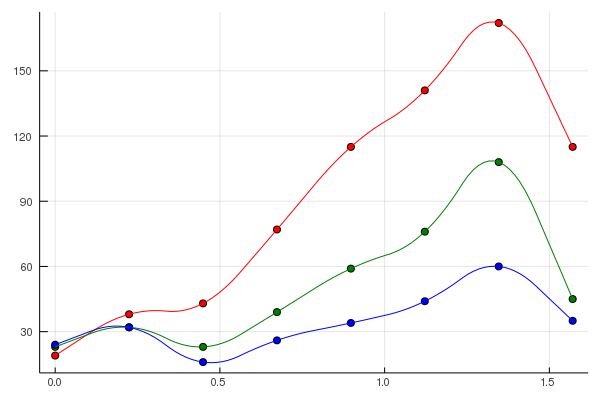
\includegraphics[scale=0.3]{../src/escape_time_algorithm/results/interpolation.png}\hfill
		\includegraphics[scale=1.3]{../src/escape_time_algorithm/results/colour_palette_100x100.png}
	}
	\subfigure[\label{subfig:Color2}Interpolación en el espacio RGB y degradado generado.]{
		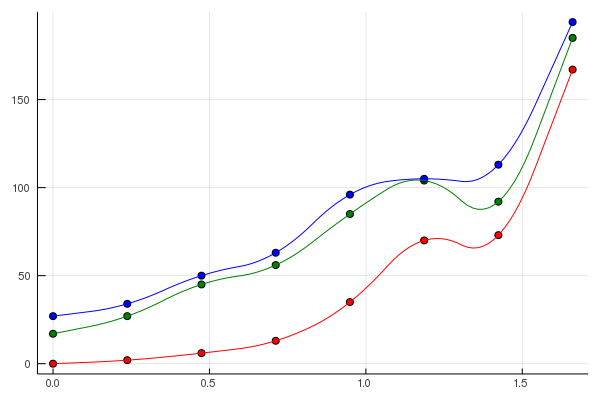
\includegraphics[scale=0.3]{../src/curvature_estimation/Burning_Ship/results/interpolation.png}
		\includegraphics[scale=1.3	]{../src/curvature_estimation/Burning_Ship/results/colour_palette_100x100.png}
	}
	\caption{Paletas de colores.}
	\label{fig:Paleta de Colores}
\end{figure}

La selección de gradiente es una de las elecciones artísticas más criticas para crear una buena imagen fractal. La selección de color puede enfatizar una parte de una imagen fractal mientras desestima otra. En casos extremos, dos imágenes con los mismos parámetros fractales, pero diferentes esquemas de color parecerán totalmente diferentes.

Con el algoritmo y los términos ahora definidos, todo lo que queda es ilustrar los resultados de algunas combinaciones de opciones.

La primer imagen, \textit{At the C-shore} (Figura \ref{fig:At the C-shore}), esta basada en la función 
\[ f(z) = \sqrt{(1-i)z-1}. \]

\begin{figure}[!hbtp]
\centering

\includegraphics[scale=0.5]{../src/curvature_estimation/A_the_C-shore/results/A_the_C-shore_12_960x540.png}
\caption{At the C-shore.}
\label{fig:At the C-shore}
\end{figure}

La iteración limite para el calculo de la curvatura es $N_{max} = 12$, y la paleta de colores es la mostrada en la Figura \ref{subfig:Color1}. \vspace{24pt}

\newpage
La imagen, \textit{i of the Storm} (Figura \ref{fig:i of the Storm}), esta basada en la función 
\[ f(z) = \frac{(1-i)z^4 + (7+i)z}{2z^5 + 6}. \]

\begin{figure}[!hbtp]
\centering
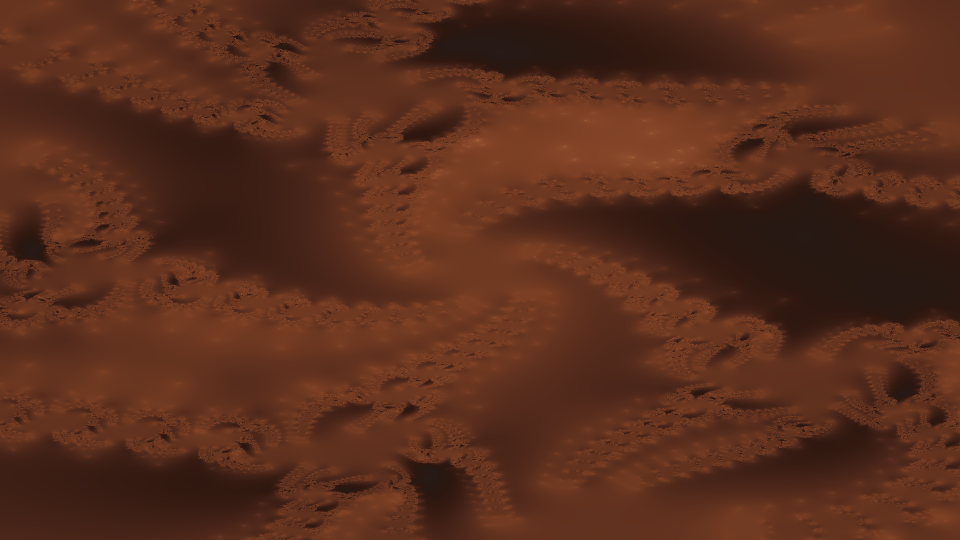
\includegraphics[scale=0.5]{../src/curvature_estimation/i_of_the_Storm/results/i_of_the_Storm_12_960x540.png} 
\caption{i of the Storm.}
\label{fig:i of the Storm}
\end{figure}

La iteración limite para el calculo de la curvatura es $N_{max} = 12$, y la paleta de colores es la mostrada en la Figura \ref{subfig:Color1}. \vspace{24pt}

\newpage
La siguiente imagen, \textit{i belong to U} (Figura \ref{fig:i belong to U}), esta basada en la función
\[ f(z) = \frac{(1-i)z^6 + (7+i)z}{2z^5 + 6}. \]

\begin{figure}[!hbtp]
\centering
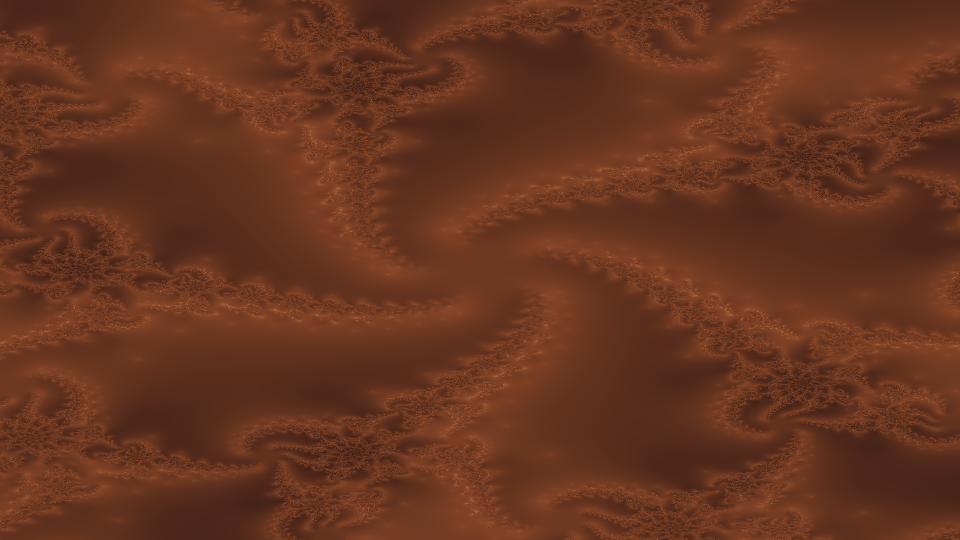
\includegraphics[scale=0.5]{../src/curvature_estimation/i_belong_to_U/results/i_belong_to_U_12_960x540.png} 
\caption{i belong to U.}
\label{fig:i belong to U}
\end{figure}

La iteración limite para el calculo de la curvatura es $N_{max} = 12$, y la paleta de colores es la mostrada en la Figura \ref{subfig:Color1}. \vspace{24pt}

\newpage
Ahora pasemos a algo mas conocido, \textit{el Conjunto de Mandelbrot} (Figura \ref{fig:Mandelbrot Set}). Este fractal esta basado en la función
\[ f(z, c) = z^2 + c. \]
El procedimiento para generar este fractal fue mencionado anteriormente.

\begin{figure}[!hbtp]
\centering
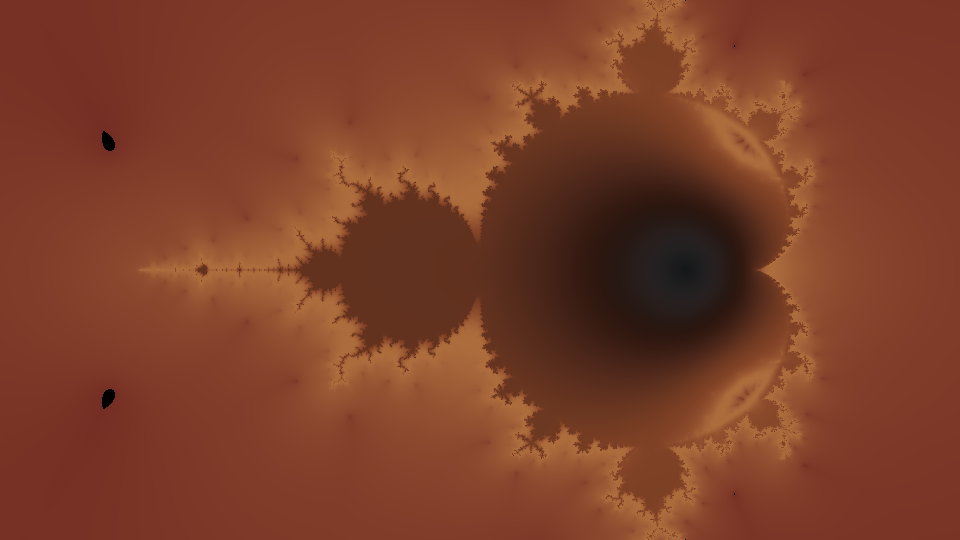
\includegraphics[scale=0.5]{../src/curvature_estimation/Mandelbrot_Set/results/MandelbrotSet_32_960x540.png} 
\caption{Mandelbrot Set.}
\label{fig:Mandelbrot Set}
\end{figure}

La iteración limite para el calculo de la curvatura es $N_{max} = 32$, y la paleta de colores es la mostrada en la Figura \ref{subfig:Color1}. \vspace{24pt}

\newpage
La ultima imagen, \textit{Burning Ship} (Figura \ref{fig:Burning Ship}), esta basada en la función
\[ f(z, c) = ( \abs{Re(z)} + i\abs{Im(z)} )^2 + c. \]
El procedimiento es el mismo que se utilizo para el Conjunto de Mandelbrot.

\begin{figure}[!hbtp]
\centering
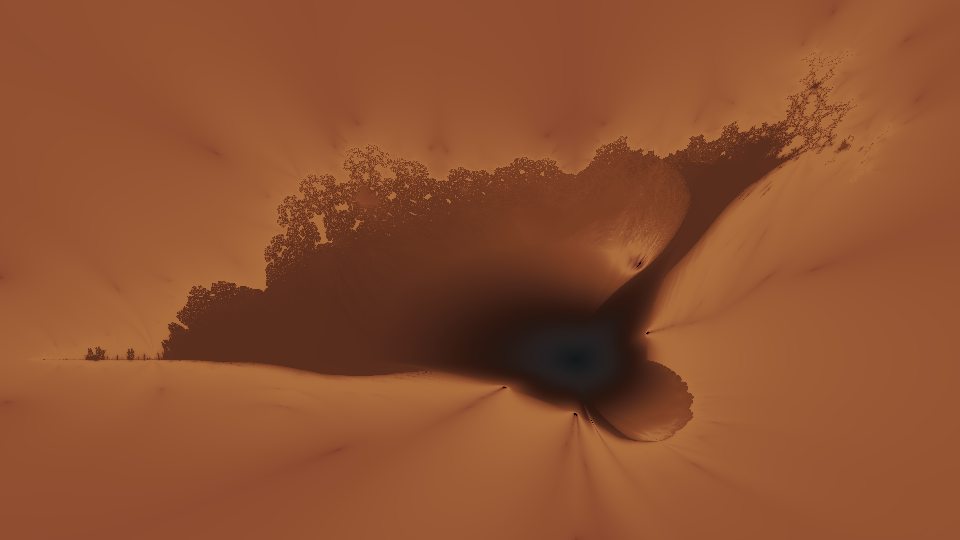
\includegraphics[scale=0.5]{../src/curvature_estimation/Burning_Ship/results/Burning_Ship_32_960x540.png} 
\caption{Burning Ship.}
\label{fig:Burning Ship}
\end{figure}

La iteración limite para el calculo de la curvatura es $N_{max} = 32$, y la paleta de colores es la mostrada en la Figura \ref{subfig:Color2}.

\newpage
Tanto el programa como las imágenes antes mostradas pueden ser encontradas en el siguiente enlace: 
\begin{center}
\url{https://github.com/JacobHdez/Fractal_Coloring}
\end{center}

%\newpage
\addcontentsline{toc}{section}{Referencias}
\begin{thebibliography}{5}
	\bibitem{Fractal Art}
	P. D. SISSON
	``\textit{Fractal art using variations on escape time algorithms in the complex plane}''
	Louisiana State University in Shreveport, USA
	
	\bibitem{Coloring Algorithms}
	Javier Barrallo \& Damien M. Jones
	``\textit{COLORING ALGORITHMS FOR DYNAMICAL SYSTEMS IN THE COMPLEX PLANE}''
	The University of the Basque Country, 2009 San Sebastián. SPAIN
	
	\bibitem{Coloring Techniques}
	Jussi Härkönen
	``\textit{On Smooth Fractal Coloring Techniques}''
	Abo Akademi University, 2007
	
	\bibitem{Fractals Everywhere}
	Michael F. Barnsley
	``\textit{FRACTALS EVETYWHERE}''
	Academic Press, 1998
\end{thebibliography}

\end{document}
